\documentclass[tikz,border=10pt]{standalone}
% No extra TikZ libraries needed.
\begin{document}
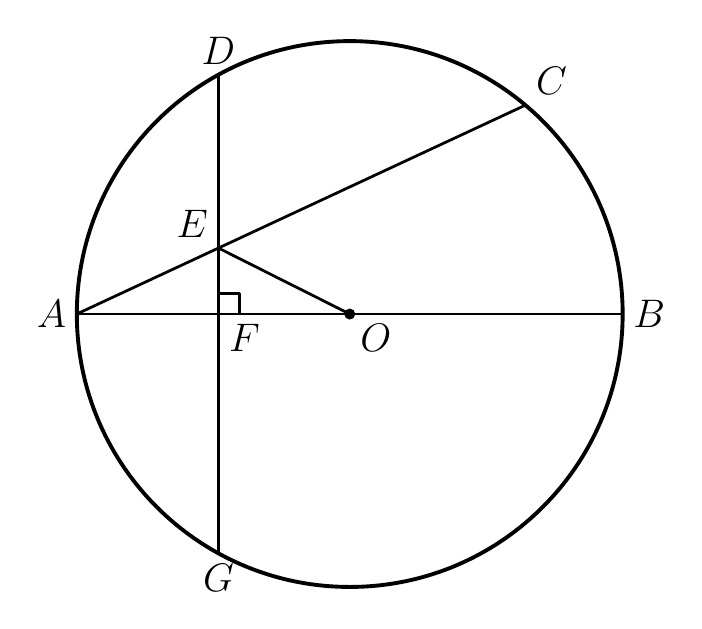
\begin{tikzpicture}[line join=round, line width=1.0pt]
  % Coordinates in cm, origin at O. Scale s = 0.017621 units/px, y flipped.
  \coordinate (O) at (0,0);
  \coordinate (A) at (-3.467,0);
  \coordinate (B) at (3.467,0);
  \coordinate (C) at (2.232,2.653);
  \coordinate (D) at (-1.667,3.039);
  \coordinate (G) at (-1.667,-3.039);
  \coordinate (F) at (-1.667,0);
  \coordinate (E) at (-1.667,0.838);

  % Circle centred at O, radius 196.7 px (heavier than the other strokes)
  \draw[line width=1.4pt] (O) circle (3.466);

  % Diameter AB
  \draw (A) -- (B);

  % Chord DG through E and F
  \draw (D) -- (G);

  % Chord AC through E
  \draw (A) -- (C);

  % Segment EO
  \draw (E) -- (O);

  % Right-angle mark at F (15 px square, inside quadrant above AB, right of DG)
  \draw (-1.403,0) -- (-1.403,0.264) -- (-1.667,0.264);

  % Dot at O (enlarged); no dot at E
  \fill (O) circle (0.07);

  % Labels
  \node[left, font=\fontsize{14.5}{17.4}\selectfont] at (A) {$A$};
  \node[right, font=\fontsize{14.5}{17.4}\selectfont] at (B) {$B$};
  \node[above right, font=\fontsize{14.5}{17.4}\selectfont] at (C) {$C$};
  \node[above, font=\fontsize{14.5}{17.4}\selectfont] at (D) {$D$};
  \node[above left, font=\fontsize{14.5}{17.4}\selectfont] at (E) {$E$};
  \node[below right, font=\fontsize{14.5}{17.4}\selectfont] at (F) {$F$};
  \node[below, font=\fontsize{14.5}{17.4}\selectfont] at (G) {$G$};
  \node[below right, font=\fontsize{14.5}{17.4}\selectfont] at (O) {$O$};
\end{tikzpicture}
\end{document}